\documentclass[11pt,a4paper]{report}
\usepackage[utf8]{inputenc}
\usepackage{amsmath}
\usepackage{amsfonts}
\usepackage{amssymb}
\usepackage{graphicx}
\usepackage{caption}
\usepackage{float}
\usepackage{natbib}
\usepackage{url}
\usepackage{mathtools}

% For displaying results
\usepackage{setspace}
\usepackage{pdflscape}
\usepackage{listings}
\usepackage{xcolor}
\usepackage{color}
\definecolor{mygreen}{rgb}{0,0.7,0.3}

\lstdefinestyle{base}{
  language=bash,
  basicstyle=\tiny,
  moredelim=**[is][\color{mygreen}]{@}{@},
  moredelim=**[is][\color{blue}]{\$}{\$},
  moredelim=**[is][\color{red}]{\{}{\}}
}

\makeatletter
\newcommand{\srcsize}{\@setfontsize{\srcsize}{1.4pt}{1.4pt}}
\makeatother

\lstdefinestyle{special}{
  language=bash,
  basicstyle={\ttfamily\srcsize},
  moredelim=**[is][\color{mygreen}]{@}{@},
  moredelim=**[is][\color{blue}]{\$}{\$},
  moredelim=**[is][\color{red}]{\{}{\}}
}

% Commands
\newcommand{\seq}{S} % sequence
\newcommand{\str}{P} % structure
\newcommand{\ens}{\mathcal{\str}} % structure ensemble
\newcommand{\ensAll}{\ens_{\text{all}}} % ensemble of all structures
\newcommand{\en}{E} % Energy
\newcommand{\parr}{Z} % Partition function
\newcommand{\parrall}{\parr_{\ŧext{all}}} % partition function of ensemble of all structures
\newcommand{\parrun}{\parr_{i,j}^u} % partition function of unpaired region [i,j]


\title{Prediction of non-related RNA-RNA interactions}
\date{\today}
\author{Rick Gelhausen}

\begin{document}
\maketitle
\section*{Introduction}
IntaRNA is an algorithm to predict interactions of bacterial sRNA with a target mRNA. An RNA molecule is transcribed from a large part of DNA. There are two classes of RNA, the coding RNA (cRNA) and the non-coding RNA (ncRNA). The cRNA is involved in the translation into proteins. For example the messenger RNA that carries informations to encode proteins. The ncRNA performs different functions in the cell. In the cRNA mainly the composition of the sequence is important, whereas the function of a ncRNA is mainly related to its structure.\\
The bacterial small RNAs used by IntaRNA, are highly structured small-chained ncRNAs produced by bacteria. They can have multiple functions, such as the modification of the function of proteins or regulate gene creation by binding to mRNA.\\
The RNA molecules are represented as a sequence $\seq\in {A,C,G,U}^*$. $s_{i}...s_{j}$ represents a subsequence of $\seq$ such that $s \subseteq \seq$. The sequences are usually ordered from the left $5^\prime$ end to the right $3^\prime$ end.\\
\begin{figure}[H]
\centering
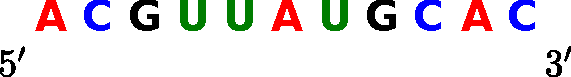
\includegraphics[scale=1]{seqExample.pdf}
\caption{RNA sequence $\seq$}
\end{figure}
\noindent
These sequences can be folded into structures that determine the function of an RNA molecule.\\
An RNA structure $\str$ of $\seq$ is a set of base pairs.
\begin{equation*}
\str\subseteq \{(i,j)\mid 1 \leq i < j \leq n, \seq_i \text{ and } \seq_j \text{ complementary}\},
\end{equation*}
where n = $\mid \seq \mid$ and the degree of $\str$ is atleast one.
As the prediction of tertiary structures is a hard problem, secondary structures are used instead.
There are different types of RNA structures. Nested structures that contain no pseudoknots and crossing structures containing pseudoknots, as shown in Figure \ref{Nested}. Pseudoknots are, as the name suggests, no real knots in the tertiary structure, but cause problems in the secondary structure representation.
\begin{figure}[H]
\centering 

\includegraphics[scale=0.6]{NestedCrossing.pdf}
\caption{Linear Feynman Diagrams of a nested and a crossing structure.}
\label{Nested}
\end{figure}
\noindent
The structure is created by bases forming base-pairs by hydrogen bonds. Due to their high binding strength G-C, A-U and G-U are the most common base pairs.\\
\begin{figure}[H]
\centering
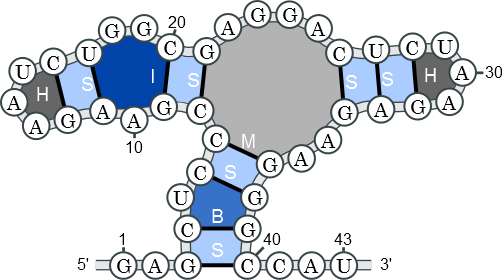
\includegraphics[scale=0.5]{structure-loops.png}
\caption{Overview of structure elements. \citep{ELearn}}
\label{Structure}
\end{figure}
\noindent
There are different structural elements that are formed by the binding of base pairs. These elements are the hairpin loops (H), stackings (S), internal/bulge loops (I/B) and multiloops (M), as shown in figure \ref{Structure}.
A secondary structure is composed of these structural elements.
The ensemble of all structures is denoted $\ensAll$.\\
IntaRNA has different restrictions to reduce the complexity of the algorithm, to make it applicable in practice. One strong restriction is that the target region is single stranded and the loops are no longer than 16 nucleotides.\\
In this work we remove these restrictions to allow structures in the target region. We will first introduce further notions and the McCaskill algorithm \citep{McCaskill} used to calculate partition functions and probabilities. Then we will introduce the update recursions of the IntaRNA algorithm to allow structures in the target region.\\
\section*{Energy Model and Probabilities}
IntaRNA uses energy minimization to find an optimal solution.
The underlying energy model is the Nearests Neighbor Model. It states that the vertical stacking of base pairs  gives the largest contribution to the stability of the system. It allows the calculation of a free energy estimate for a RNA secondary structure. The lower the free energy the more energy has to be invested to disrupt the system. A structure is more stable, the lower the free energy. This means that the stablest structure is the minimum free energy structure (mfe). As the free energy is hard to calculate, the usage of energy differences is customary. The free energy is calculated with respect to the unstructured open chain.\\
%TODO % MISSING LINK
The boltzmann distribution is, according to the maximum entropy principal, the best probability distribution for the calculation of structure or base pair probabilities. It gives us a huge information gain, with a low information content. We therefor calculate probabilities according to their boltzmann weights.
\begin{equation*}
w(\str) = \exp(\frac{-\en(\str)}{RT}),
\end{equation*}
where $\en$ is a specific energy of a structure $\str$, R is the gas constant used to calculate the energy for a single molecule and T is the temperature.\\\\ %TODO check this\\
Using these boltzmann weights we can calculate the partition function $\parr$. $\parr$ is the sum over all boltzmann weights for all structures $\str$.
\begin{equation*}
\parr = \sum\limits_{\str\in\ens} w(\str)
\end{equation*}
$\parr$ is required in the calculation of structure and base pair probabilities. These probabilities are calculated in the thermodynamic equilibrium. This means that there are no observable changes on a macroscopic level. Multiple different probabilities can be calculated. Such as the probability of a structure to be formed.\\
\begin{align*}
Pr[\str|\ens] = \frac{w(\str)}{\parr}
\end{align*}\\
This way the k most probable mfe structures can be calculated. As the underlying energy model is an estimation and simplification of the truth, the structure with the highest probability does not have to be the functional structure, but it is safe to assume that the best structure is among the most probable structures.\\
It is also possible to calculate the probability that a certain base pair appears.\\
\begin{align*}
Pr[(i,j)|\ens] = \sum\limits_{(i,j) \in \str} \frac{w(\str)}{\parr}
\end{align*}\\
The probability that base pair $(i,j)$ occurs. These base pair probabilities can be represented in a dot plot and give a good overview how the most probable structure can look like, because the most probable base pairs are likely contained in the most probable structures.\\
Furthermore the probability that a given region of a structure is unpaired can be determined.\\
\begin{align*}
Pr_u [i,j] = \frac{Z_{i,j}^{u}}{Z},
\end{align*}\\
where $Z_{i,j}^{u}$ is the partition function of all structures with subsequence $[i,j]$ unpaired.
\begin{equation*}
\parrun = \sum\limits_{\str \subset \ens_{i,j}^u} w(\str) = \parr(\ens_{i,j}^u)
\end{equation*}
where $\ens_{i,j}^u$ is the ensemble of all structures that are unpaired between i and j.
\begin{equation*}
\ens_{i,j}^u = \{\str \mid \nexists (k,l) \in \str : i\leq k \leq j \text{ or } i \leq l \leq j \} \subseteq \ensAll
\end{equation*}
The unpaired probability is very important, as it allows the calculation of the accessibility of single stranded regions.
\newpage
\section*{McCaskill}
\subsection*{Preliminaries}
The McCaskill algorithm is used to calculate the partition function Z for a given sequence S, which can be used to compute probabilities.\\
The basic idea is to use an algorithm, similar to the Zuker algorithm, to sum up the boltzmann weights for all possible structure. The important part is to count every structure only once, which requires the creation of a special multiloop case.\\
There are four matrices required in the algorithm.
\begin{align*}
Q_{i,j} = Z_{\mathcal{S}_{i,j}} && Q_{i,j}^m &= Z_{\mathcal{S}_{i,j}^{1bd}}^m\\
Q_{i,j}^b = Z_{\mathcal{S}_{i,j}}^b && Q_{i,j}^{m1} &= Z_{\{P\in \mathcal{S}_{i,j}^{1bd}| \text{only one exterior bp in P}\}}^m
\end{align*}
$Q_{i,j}$ contains the summed boltzmann weights for all structures which only contain bonds in range $[i,j]$. $Q_{i,j}^b$ has the additional property that $(i,j)$ forms a base pair. $Q_{i,j}^{m}$ has the additional property that there is atleast one base pair in range $(i,j)$. $Q_{i,j}^{m1}$ has the property that there is exactly one base pair within $(i,j)$. The final result $Z=Z_{\mathcal{S}_{all}}$ is contained in $Q_{1,\mid N\mid}$.\\ %TODO Reformulate sounds wacky\\
The decomposition has to be disjoint and independent to ensure that every structure is only counted once. This requires a change in the multiloop split case of the Zuker algorithm, as it is an ambiguous decomposition. Therefore the matrix $Q_{i,j}^{m1}$ is introduced, where the multiloop split is always done at the last bond. This ensures an unambiguous decomposition.\\
\begin{figure}[H]
\centering
\captionsetup{justification=centering,margin=2cm}

\includegraphics[scale=1]{ASplit.pdf}
\caption{Ambiguous multiloop split. The split could be done at k1, k2 or k3.}
\end{figure}
\subsection*{Matrices}
In the following equations a, b and c represent energy contributions of multiloops. This is a simplification of the real energy contributions of multiloops, because the real energy contribution computation is too complex. a denotes the energy contribution for closing the multiloop. b denotes the contribution for enclosed helices and c denotes the contribution for enclosed unpaired bases. The energy contribution for hairpin loops is denoted as $eH(i,j)$ and the contribution for stacking, internal and bulge loops are denoted as $eSBI(i,j,i^\prime,j^\prime)$.\\\\
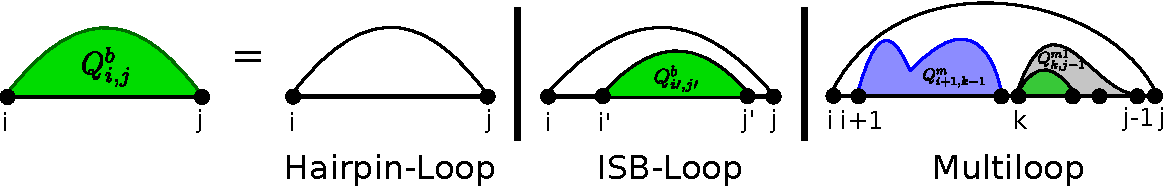
\includegraphics[scale=0.65]{QB.pdf}\\
\begin{align}
Q_{ij}^b = \sum \begin{cases}
					e^{\frac{-eH(i,j)}{RT}}\\
					\sum\limits_{i<i^{\prime} <j^{\prime} <j}(Q_{i^{\prime}, j^{\prime}}^b \cdot e^{\frac{-eSBI(i,j,i^{\prime},j^{\prime})}{RT}})\\
					\sum\limits_{i < k < j} (Q_{i+1,k-1}^m \cdot Q_{k, j-1}^{m1} \cdot e^{\frac{-a}{RT}})
				\end{cases}
\end{align}
In the $Q_{i,j}^b$ matrix, we add up the energy contributions for the different possible structure elements.\\
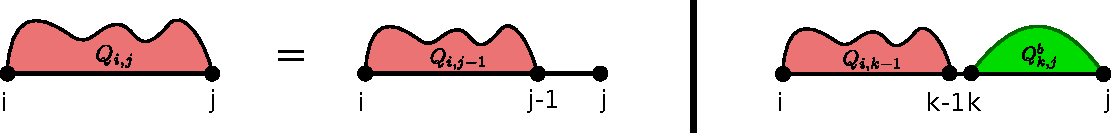
\includegraphics[scale=0.65]{Q.pdf}
\begin{align}
Q_{i,j} = Q_{i,j-1}+ \sum\limits_{i \leq k < j} Q_{i,k-1}\cdot Q_{k,j}^b
\end{align}
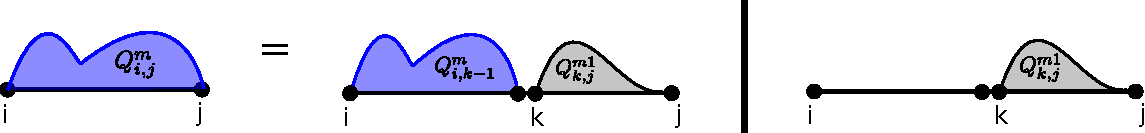
\includegraphics[scale=0.65]{QM.pdf}
\begin{align} \label{eq:1}
Q_{i,j}^m = \sum\limits_{i\leq k < j} (Q_{i,k-1} + e^{\frac{-(k-i)c}{RT}}) \cdot Q_{kj}^{m1}
\end{align}
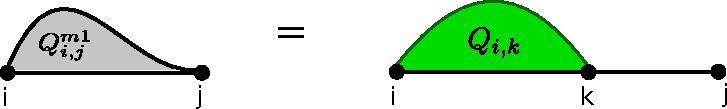
\includegraphics[scale=0.65]{QM1.pdf}
\begin{align}
Q_{kj}^{m1} = \sum\limits_{i< k \leq j} Q_{i,k}^b \cdot e^\frac{-b}{RT} \cdot e^\frac{-(j-k)c}{RT}
\end{align}
The initialization for the matrices $Q_{i,j}^b$, $Q_{i,j}^m$ and $Q_{i,j}^{m1}$ is 0. For the single-stranded sequence there is no base, therefore there will not be an entry in these matrices. $Q_{i,j}$ is initialized with 1 as it covers the single-stranded sequence.\\
\subsection*{Base pair probabilities:}
The probabilities for unpaired bases can be calculated using the McCaskill recursions. There are three possible locations for a base pair $(k,l)$.\\
\begin{enumerate}
\item $(k, l)$ is an external base pair:
\begin{figure}[H]
\centering
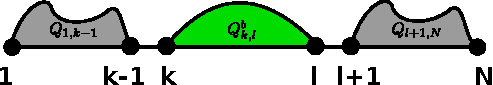
\includegraphics[scale=1]{BPP1.pdf}
\end{figure}
\begin{equation*}
p_{kl}^E = \frac{Q_{1,k-1} \cdot Q_{k,l}^b \cdot Q_{l+1,n}}{Q_{1,n}}
\end{equation*}
\item $(k, l)$ limits a stacking, bulge- or interior loop closed by bp $(i,j)$, where $i < k < l < j$.
\begin{figure}[H]
\centering

\includegraphics[scale=0.6]{BPP2.pdf}
\end{figure}
\begin{equation*}
p_{kl}^{SBI} (i,j) = p_{ij} \frac{\exp(\frac{-eSBI(i,j,k,l)}{RT}) Q_{k,l}^b}{Q_{i,j}^b}
\end{equation*}\\\\
The probility that base pair $(i,j)$ is formed $p_{i,j}$ is computed in an outside recursion, before the computation of $p_{kl}^{SBI}$. $p_{i,j}$ is then corrected by taking the additional constraint that the loop $i,j,k,l$ is formed. The numerator of the fraction is the partition function of all structures containing bp $(k,l)$. It is corrected by the denominator $Q_{i,j}^b$ which is the partition function of all bp containing bp $(i,j)$. \\
\item $(k, l)$ closes an inner helix of a multiloop closed by bp $(i,j)$, where $i < k < l < j$.\\\\
$p_{kl}^M (i,j) = p_{ij} \cdot Pr[\text{Multiloop with inner bp } (k,l) \text{ closed by } (i,j) \mid (i,j)]$\\\\
There are again three locations for $(k,l)$ inside the multiloop:
\begin{enumerate}
\item $(k,l)$ is the leftmost base pair:
\begin{figure}[H]
\centering
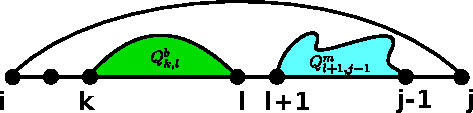
\includegraphics[scale=0.75]{BPP3.pdf}
\end{figure}
\begin{equation*}
\frac{Q_{k,l}^b \cdot Q_{l+1, j-1}^m \cdot \exp(\frac{-(a+b+(k-i-1)c)}{RT})}{Q_{i,j}^b}
\end{equation*}
\item $(k,l)$ is the middle base pair:
\begin{figure}[H]
\centering
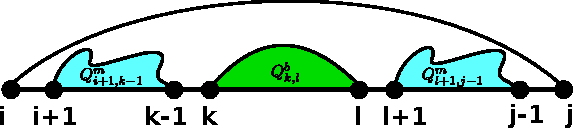
\includegraphics[scale=0.75]{BPP4.pdf}
\end{figure}
\begin{equation*}
\frac{Q_{i+1,k-1}^m \cdot Q_{k,l}^b \cdot Q_{l+1,j-1}^m \cdot \exp(\frac{-(a+b)}{RT})}{Q_{i,j}^b}
\end{equation*}
\item $(k,l)$ is the rightmost base pair:
\begin{figure}[H]
\centering
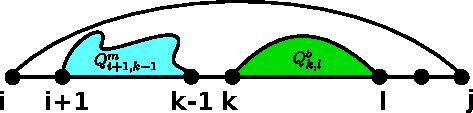
\includegraphics[scale=0.75]{BPP5.pdf}
\end{figure}
\begin{equation*}
\frac{Q_{i+1,k-1}^m \cdot Q_{k,l}^b \cdot \exp(\frac{-(a+b+(j-l-1)c)}{RT})}{Q_{i,j}^b}
\end{equation*}
\end{enumerate}
%TODO Drawing
\begin{align*}
p_{kl}^M (i,j) = \frac{p_{ij}}{Q_{i,j}^b} &\cdot (Q_{k,l}^b \cdot Q_{l+1, j-1}^m \cdot \exp(\frac{-(a+b+(k-i-1)c)}{RT})\\ &+ Q_{i+1,k-1}^m \cdot Q_{k,l}^b \cdot Q_{l+1,j-1}^m \cdot \exp(\frac{-(a+b)}{RT})\\ &+ Q_{i+1,k-1}^m \cdot Q_{k,l}^b \cdot \exp(\frac{-(a+b+(j-l-1)c)}{RT}))
\end{align*}
\end{enumerate}
The overall probability for a base pair $(k,l)$ is denoted:\\
\begin{equation*}
p_{kl} = p_{kl}^E + \sum\limits_{i<k,l<j} p_{kl}^{SBI}(i,j) + \sum\limits_{i<k,l<j} p_{kl}^M (i,j)
\end{equation*}
\subsection*{Probabilities of unpaired regions:}
A very important concept for RNA-RNA interaction prediction is the calculation of the probability of unpaired regions, as unpaired regions are possible targets for interactions.\\
These probabilities $Pr_u[i,j]$ can again be calculated using the McCaskill recursions.\\
\begin{equation*}
Pr_u[i,j] = \frac{Z_{\mathcal{P}_{i,j}^u}}{Z_{\mathcal{P}_{all}}}
\end{equation*}
The probability that region $[i,j]$ is unpaired, where $\mathcal{P}_{i,j}^u$ is the set of structures where region $[i,j]$ is unpaired and $\mathcal{P}_{all}$ the set of all structures for a given sequence.\\
There are two different locations for an unpaired region it is either exterior or enclosed. An exterior region is enclosed by no base pairs. The enclosed region is either enclosed by a hairpin, an interior/bulge loop or a multiloop. Using a disjoint decomposition of $\mathcal{P}_{i,j}^u$ the different cases can be viewed independantly.\\
\begin{description}
\item[Case I] $[i,j]$ is exterior:\\
\begin{figure}[H]
\centering
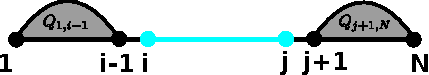
\includegraphics[scale=0.75]{UNO.pdf}
\end{figure}
\begin{equation*}
Pr_u[i,j\mid exterior] = \frac{Q_{1,i-1}\cdot 1 \cdot Q_{j+1,N}}{Q_{1,N}}
\end{equation*}
where N is the length of the sequence and 1 is the boltzmann weight of the unpaired region.
The multiplication is justified as this is an independent decomposition of the sequence.\\ 
\item[Case II] $[i,j]$ is enclosed by bp $(p,q)$:\\
\begin{equation*}
Pr_u[i,j\mid enclosed] = \sum\limits_{p<i,j<q} \frac{Pr[(p,q)]}{Q_{p,q}^b} \cdot Q_{i,j}^{pq}
\end{equation*}
where $Pr[(p,q)]$ is the probability that $(p,q)$ forms a base pair. $Q_{p,q}^b$ is the partition function of all structures that form are enclosed by $(p,q)$ and $Q_{i,j}^{pq}$ is the partition function of all structures that have a base pair $(i,j)$ enclosed by a bp $(p,q)$.\\
$Q_{i,j}^{pq}$ is composed of the sum over the different cases of structural elements.\\
\begin{enumerate}
\item \underline{Hairpin Loop:}\\
\begin{figure}[H]
\centering
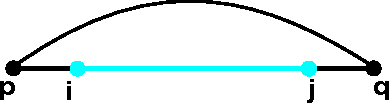
\includegraphics[scale=0.75]{UHPL.pdf}
\end{figure}
\begin{equation*}
e^\frac{-eH(p,q)}{RT}
\end{equation*}
\item \underline{Stacking, Internal- and Bulge Loop:}\\
\begin{figure}[H]
\centering

\includegraphics[scale=0.75]{USBIL.pdf}
\end{figure}
\begin{equation*}
\sum_{\substack{p < i \leq j <k\\ or\\ l < i \leq j < q}} e^\frac{-eSBI(p,q,k,l)}{RT} \cdot Q_{k,l}^b
\end{equation*}
\item \underline{Multiloop:}\\
\begin{figure}[H]
\centering

\includegraphics[scale=0.75]{UML.pdf}
\end{figure}
\begin{align*}
\sum\limits_{p<i\leq j<q} &\; \quad Q_{p+1,i-1}^{m2} \cdot e^\frac{-(q-i)c}{RT}\\
&+Q_{p+1,i-1}^m \cdot e^\frac{-(j-i+1)c}{RT} \cdot Q_{j+1,q-1}^m\\
&+e^\frac{-(j-p)c}{RT} \cdot Q_{j+1,q-1}^{m2}\\
\text{with } Q_{i,j}^{m2} &= \sum\limits_{p<k<q} Q_{p,q}^m \cdot Q_{k+1,q}^{m1}
\end{align*}
where $Q^{m2}$ ensures that we have atleast two helices.\\
\end{enumerate}
The probability that $[i,j]$ is unpaired is:
\begin{align*}
Pr_u[i,j] &= Pr_u[i,j\mid exterior] + Pr_u[i,j\mid enclosed]\\
&=\frac{Q_{1,i-1}\cdot 1 \cdot Q_{j+1,N}}{Q_{1,N}}
+\sum\limits_{p<i,j<q} \frac{Pr[(p,q)]}{Q_{p,q}^b} \cdot Q_{i,j}^{pq}
\end{align*}
\end{description}
\newpage
\section*{IntaRNA}
IntaRNA is an algorithm to predict RNA-RNA interactions of bacterial small RNAs and a target mRNA. The original version of IntaRNA is limiting the loop sizes in the target regions to 16 nucleotides and it allows neither inter, nor intra molecular base pairs in the target region.\\
There are two major components in IntaRNA that determine the quality of RNA-RNA interactions between two subsequences of sequences $\seq^1$ and $\seq^2$, the hybridisation energy $H(i,j,k,l)$ and the accessibility of the interaction site.\\
The hybridisation energy is calculated using the nearest neighbour energy model. It represents the hybridisation minimum free energy of two subsequences, where the leftmost positions of both subsequences form a base pair.\\
For simplification purposes $E_{3^\prime}^{dangle}$, $E_{5^\prime}^{dangle}$ and $E_{mm}^{term}$ will not be considered in the following recursions.\\
For subsequences  $\seq_{i}^1 ... \seq_{k}^1$ and $\seq_{j}^2 ... \seq_{l}^2$, where $\seq^1$ is ordered from $5^\prime$ to $3^\prime$ and $\seq^2$ in the reverse order:
\begin{equation*}
H(i,j,k,l) = \min\{E(\str)\mid (i,j) \in \str \wedge (k,l) \in \str\}
\end{equation*}
The hybridization energy is calculated with a Zuker-like recursion.\\
\begin{equation*}
H(i,j,k,l) = \min \begin{cases}
					E_{init}\\
    				\quad\text{: if } \seq_{i}^1, \seq_{j}^2\text{ can pair, } i = k \text{ and } j = l,\\
    				\min\limits_{r,s} \{E^{loop}(i,j,r,s) + H(r,s,k,l)\}\\
    				\quad \text{: if } \seq_{i}^1, \seq_{j}^2\text{ can pair, }i\neq k \text{ and } j\neq l,\\
   					\infty\\
   					\quad\text{: otherwise.}\\
				\end{cases}\\
\end{equation*}
where $E^{loop}(i,j,k,l)$ represents the energy contribution of the loop formed by the base pairs $(i,j)$ and $(k,l)$.\\
The accessibility represents the energy required to make the interaction site single-stranded. It is calculated as the energy difference between the energy of the ensemble of all structures that can be formed by $\seq$ and the energy of the ensemble of all structures, where the interaction site is single-stranded.\\
This energy difference $ED(i,j)$ is computed using a partition function approach as introduced by \citep{McCaskill}.\\
The free energy of the ensemble $\ens$ is\\
\begin{equation*}
E^{ens}(\ens) = -RT \cdot ln(\parr_\ens)
\end{equation*}
It follows that $ED(i,k)$ is\\
\begin{equation*}
ED(i,k) = E^{ens}(\ens_{i,k}^{unpaired}) - E^{ens}(\ens)
\end{equation*}
Figure \ref{contribution} shows the energy contributions considered in the original IntaRNA recursions.
\begin{figure}[H]
\centering
\captionsetup{justification=centering,margin=2cm}
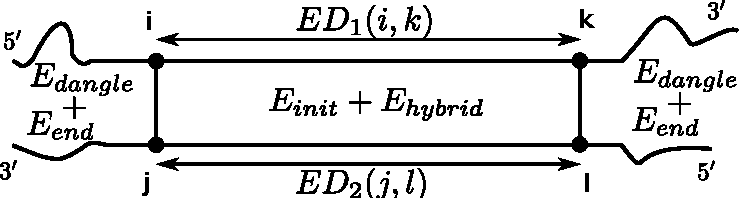
\includegraphics[scale=0.75]{energy.pdf}
\caption{The energy contributions needed in the original IntaRNA recursions.}
\label{contribution}
\end{figure}
\noindent
Both the accessibility and the hybridisation energy are combined to form the extended hybridisation energy.
The extended hybridisation energy of a specific hybridisation between $\seq^1_i ... \seq^1_k$ and $\seq^2_j...\seq^2_l$ is defined by:
\begin{equation*}
C(i,j,k,l) = \begin{cases}
					H(i,j,k,l) + ED_1(i,k) + ED_2(j,l)\\
					\quad\text{: if } \seq_{i}^1, \seq_{j}^2\text{ can pair, }i\neq k \text{ and } j\neq l,\\
   					\infty \\
   					\quad\text{: otherwise.}\\
			\end{cases}
\end{equation*}
\subsection*{Motivation}
Due to the strong restrictions to the interaction site by IntaRNA, many different structures, that exist in nature as seen in Figure \ref{nowPos}, cannot be predicted.
\begin{figure}[H]
\centering
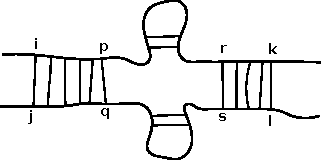
\includegraphics[scale=1.25]{PossibleStructs.pdf}
\caption{Predicted structures containing multi-loops.}
\label{nowPos}
\end{figure}
\noindent
This is because we disallow intra-molecular base pairs in the target regions. Our aim is to change the IntaRNA recursions to allow structure in the interaction site.
This will create different multi-loop cases and leave us with a new matrix $H^m(i,j,k,l)$.\\
By incorporating structure in the interaction site, we have to introduce a new energy $ES(i,k)$ which denotes the energy contribution of the structure present in the interval $]i,k[$.\\
\begin{figure}[H]
\centering
\captionsetup{justification=centering,margin=2cm}
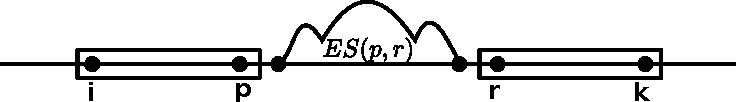
\includegraphics[scale=0.75]{EStructure.pdf}
\caption{The energy contribution of the structure on the interaction site.}
\end{figure}
\noindent
The $ES(p,r)$ is calculated similar to the free energy of the structure ensemble, under the condition that the structure is in the interval $]p,r[$ excluding the bases $p$ and $r$ that are forming base pairs with $q$ and $s$ respectively.\\ 
\begin{equation*}
ES(p,r) = -RT \cdot ln(Q_{p+1,r-1}^{m})
\end{equation*}
where $Q^m$ [\ref{eq:1}] denotes the same matrix used in the McCaskill recursion \citep{McCaskill}. It ensures atleast one base pair in the interaction site.\\
\begin{figure}[H]
\centering
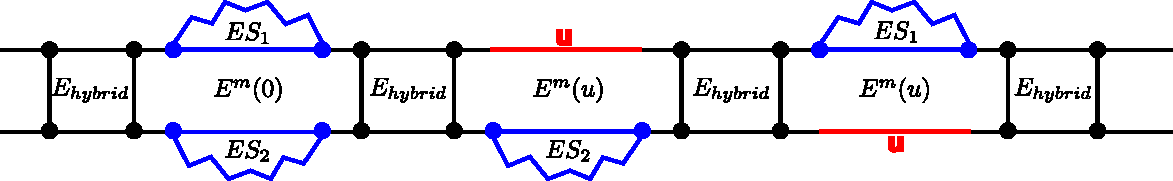
\includegraphics[scale=0.6]{Energy2.pdf}
\caption{The different multi-cases with their associated energy contributions.}
\end{figure}
\noindent
We have to consider the hybridisation energy, the structural energy and the multi-loop energies for each part. 
Furthermore, we will introduce a new energy function $E^m (u)$, which represents the energy contributions for the multi-loop.
\begin{equation*}
E^m(u) = a + b + c\cdot u
\end{equation*}
where $u$ is the number of unpaired bases enclosed by the multi-loop, $a$ is the energy contribution for closing the multi-loop, b is the energy contribution for the number of helices and $c$ is the contribution for unpaired bases $u$.\\
The usage of the simple $E^m$ energy function is justified, as all further energy contributions resulting from the structure are contained in the $ES$ values, due to the $Q^m$ matrix term.\\
Moreover, we have to analyse whether it makes more sense to add the initial energy for each structural part as a penalty or to add it once for the entire sequence.\\
Another idea is to replace the energy contribution for the closing pair of the multi-loop by the initial energy term. In the Turner 2004 parameters the $a$ term is given by $9.3$ kcal/mol and the initial energy $E_{init}$ is $4.1$ kcal/mol.
%TODO DISCUSS
\subsection*{Multiloop cases}
To introduce structure in the interaction site, we have to distinguish the different multiple cases. The structure is either in $\seq^1$, in $\seq^2$ or in both.\\
\begin{enumerate}
\item \textbf{Structure in $\seq^1_{p+1} ... \seq^1_{r-1}$:}\\
The interval $]p,r[$ is structured while the intervals $[i,p]$, $[r,k]$ and $[j,l]$ are free, with $i \leq p < q \leq k$ and $j \leq r < s \leq l$, under the condition that $(i,j)$, $(k,l)$, $(p,q)$ and $(r,s)$ form a base pair.\\
To reduce the complexity we limit the length of the unpaired region $1 \leq s-q-1 \leq 16$. This $\leq 16$ is the same as in the interior loop length restriction.\\
\begin{figure}[H]
\centering
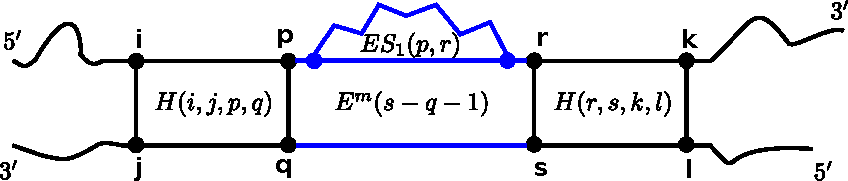
\includegraphics[scale=0.75]{RNAi1.pdf}
\end{figure}
The energy is then computed using the hybridisation energy, the ED and ES values and the contribution for closing base pairs, helices and unpaired bases.\\
\begin{align*}
E &= H(i,j,p,q) + ES_1(p,r)\\
 &+ E^m(s-q-1) + H(r,s,k,l)\\
 &+ ED_1(i,k) + ED_2(j,l)
\end{align*}
\item \textbf{Structure in $\seq^2_{q+1} ... \seq^2_{s-1}$:}\\
This case in analogous to the first case. The structure is now in the interval $]q,s[$.
\begin{figure}[H]
\centering
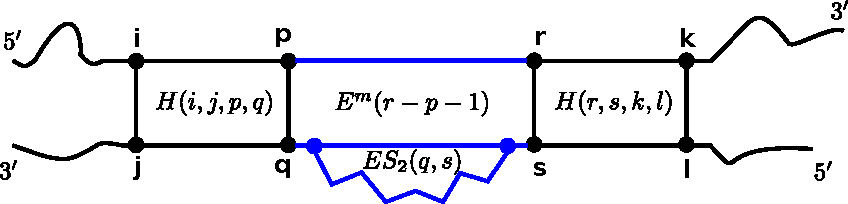
\includegraphics[scale=0.75]{RNAi3.pdf}
\end{figure}
\begin{align*}
E &= H(i,j,p,q) + E^m(r-p-1)\\
 &+ ES_2(q,s) + H(r,s,k,l)\\
 &+ ED_1(i,k) + ED_2(j,l) 
\end{align*}
\item \textbf{Structure in both subsequences:}\\
The interval $]p,q[$ and $]r,s[$ are both structured and $(i,j)$ and $(p,q)$, as well as $(r,s)$ and $(k,l)$ form base pairs, with $i \leq p < q \leq k$ and $j \leq r < s \leq l$.\\
\begin{figure}[H]
\centering
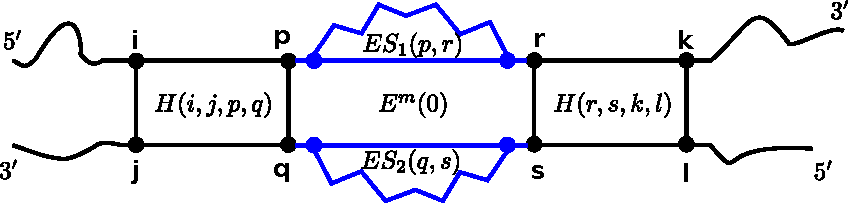
\includegraphics[scale=0.75]{RNAi2.pdf}
\end{figure}
\begin{align*}
E &= H(i,j,p,r) + ES_1(p,r) + E^m(0)\\
 & + ES_2(q,s) + H(q,s,k,l)\\
 & + ED_1(i,k) + ED_2(j,l)\\ 
\end{align*}
\end{enumerate}
Combining these cases leaves us with the new $H^m(i,j,k,l)$ matrix, which replaces the old $H(i,j,k,l)$ matrix.\\
\begin{equation*}
H^m(i,j,k,l) =  \min\begin{cases}
						E_{init}\\
						\quad\text{: Initialization energy}\\
						\min\limits_{\substack{i < r \leq k\\ j < s \leq l}} E^{loop}(i,j,r,s) + H^m(r,s,k,l)\\
						\quad\text{: Interior loop case}\\
						\min\limits_{\substack{i < r \leq k\\ j < s \leq l}}\begin{cases}
									H^m(r,s,k,l) + ES_1(i,r) + ES_2(j,s) + E^m(0)\\
									H^m(r,s,k,l) + ES_1(i,r) + E^m(r-i-1)\\
									H^m(r,s,k,l) + E^m(s-j-1) + ES_2(j,s)\\
						\end{cases}\\
						\quad\text{: Multi-loop cases}\\
   						\infty\\
			  \end{cases}\\
\end{equation*}
The $C^m(i,j,k,l)$ is analogous to the $C(i,j,k,l)$ matrix. The $H(i,j,k,l)$ entries are simply replaced by $H^m(i,j,k,l)$ entries.\\
\newpage
\subsection*{Complexity}
The newly created matrix $H^m(i,j,k,l)$ has a space complexity of $O(n^4)$ and a time complexity of $O(n^6)$ when allowing ES values in both the query and the target sequence. IntaRNA offers the option to chose between different modi, we can allow ES values in either the query sequence (--predMulti=Q), the target sequence (--predMulti=T), both sequence simultanously (--predMulti=B) or in both sequences independently (--predMulti=X). When allowing ES values in only the query or target structure or allowing ES values in both independently the complexity is reduced to $O(n^5)$. Allowing ES values in both sequences simultaneously causes $O(n^6)$ time complexity.\\
\subsection*{Results}
We tested the new IntaRNA recursion on several datasets. First, we used a structure from the Accessfold paper [\cite{doi:10.1093/bioinformatics/btv682}], shown in figure \ref{accessfold}, and we tried to reproduce the structure using our recursions. \\
\begin{figure}[H]
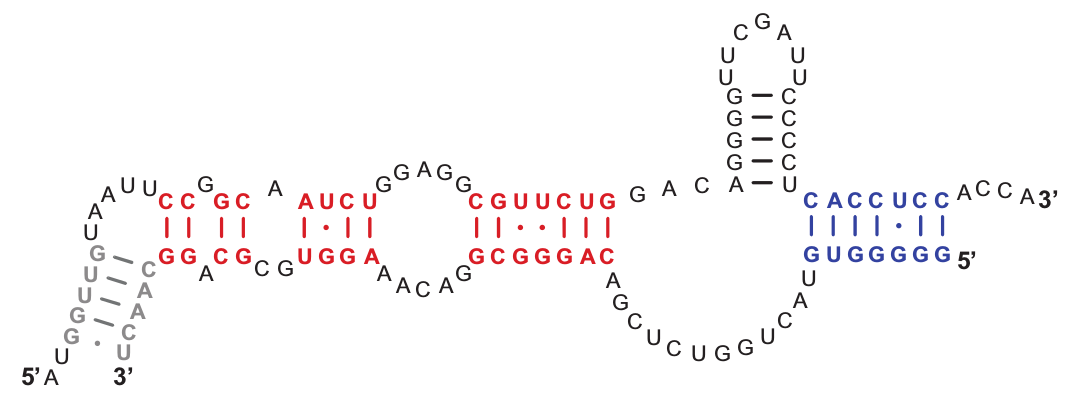
\includegraphics[scale=0.33]{Accessfold.png}
\caption{tmRNA structure. Taken from \cite{doi:10.1093/bioinformatics/btv682}.}
\label{accessfold}
\end{figure}
\noindent
The representation below shows the structure of figure \ref{accessfold} the way IntaRNA returns results. The other depictions show the output of IntaRNA using the different modi. The green regions were predicted correctly, the blue regions are missing in every result and the red regions were wrongly predicted, when comparing the output structures with the desired tmRNA structure. A base pair containing two colors indicates that the right query base formed a base pair with the wrong target base or vice versa.\\
\newpage
\begin{spacing}{0.5}
\noindent
{\tiny\texttt{>query Betaproteobacteria\_1 1-47}\\
\texttt{GGGGGUGUACUGGUCUCGACAGGGCGGACAAAGGUGCGCAGGCAACU}\\
\texttt{>target Betaproteobacteria\_2}\\
\texttt{AUGGUUGUAAUUCCGGCAAUCUGGAGGCGUUCUGGACAGGGGUUCGAUUCCCCUCACCUCCACCA}\\\\}
\end{spacing}
\begin{lstlisting}[style=base]
tmRNA structure:
target
             3                                                          61
             |                                                          |
        5'-AU     UAAUU  G   A    GGAGG       GACAGGGGUUCGAUUCCCCU       ACCA-3'
             @GGUUG@     $CC$ @GC@  @AUCU@     @CGUUCUG@         	          @CACCUCC@
             @:||||@     $||$ @||@  @|:||@     @||::|||@    	          @||||:||@
             @UCAAC@     $GG$ $CG$  @UGGA@     @GCGGGAC@    	          @GUGGGGG@
          3'-            A  CG    AACAG       AGCUCUGGUCAU                -5'
             |                                                          |
            47                                                          1
query

Results IntaRNA without multiloop recursion:
target
            28     34
             |     |
5'-AUG...GAGG       GACA...CCA-3'
             @CGUUCUG@
             @||::|||@
             @GCGGGAC@
3'-UCA...ACAG       AGCU...GGG-5'
             |     |
            26     20
query

Result of IntaRNA --pred=M --mode=E --predMulti=T --noSeed:
target
             3                                                              61
             |                                                              |
        5'-AU      AAUUCCG  A    GGAGG                 GGGUUCGAUUCCCCU       ACCA-3'
             @GGUUG@{U}       @GC@ @AUCU@     @CGUUCUG@    {GA} {CAG}               @CACCUCC@
             @:||||@{:}       @||@ @|:||@     @||::|||@    {||} {|||}               @||||:||@
             @UCAAC@{G}       {CG} @UGGA@     @GCGGGAC@    {CU} {GUC}               @GUGGGGG@
          3'-      GACG          AACAG       AGCU  G   AU                    -5'
             |                                                              |
            47                                                              1
query

Result of IntaRNA --pred=M --mode=E --predMulti=Q --noSeed:
target
            28     34
             |     |
5'-AUG...GAGG       GACA...CCA-3'
             @CGUUCUG@
             @||::|||@
             @GCGGGAC@
3'-UCA...ACAG       AGCU...GGG-5'
             |     |
            26     20
query

Result of IntaRNA --pred=M --mode=E --predMulti=X --noSeed:
target
             3                                                              61
             |                                                              |
        5'-AU      AAUUCCG  A    GGAGG                 GGGUUCGAUUCCCCU       ACCA-3'
             @GGUUG@{U}       @GC@ @AUCU@     @CGUUCUG@    {GA} {CAG}               @CACCUCC@
             @:||||@{:}       @||@ @|:||@     @||::|||@    {||} {|||}               @||||:||@
             @UCAAC@{G}       {CG} @UGGA@     @GCGGGAC@    {CU} {GUC}               @GUGGGGG@
          3'-      GACG          AACAG       AGCU  G   AU                    -5'
             |                                                              |
            47                                                              1
query

Result of IntaRNA --pred=M --mode=E --predMulti=B --noSeed:
target
             3                                                         61
             |                                                         |
        5'-AU      AAUUCCGGCAAUCUGGAGGCGUUCUGGACAGGGGUUCGAUUCCCCU       ACCA-3'
             @GGUUG@{U}                                              @CACCUCC@
             @:||||@{:}                                              @||||:||@
             @UCAAC@{G}                                              @GUGGGGG@
          3'-      GACGCGUGGAAACAGGCGGGACAGCUCUGGUCAU                   -5'
             |                                                         |
            47                                                         1
query
\end{lstlisting}
\noindent
The best result is achieved by using the ``--predMulti=T" mode, allowing ES values for the target sequence only or ``--predMulti=X" allowing ES values for the target or the query sequence. In both cases, there is one region with missing interactions and the region before the intramolecular structure should not interact.\\
The query sequence used in the Accesfold paper [\cite{doi:10.1093/bioinformatics/btv682}] was restricted to the first 47 nucleotides. We tried using the full query sequence.\\
\begin{spacing}{0.5}
\noindent
{\tiny\texttt{>query Betaproteobacteria\_1}\\
\texttt{GGGGGUGUACUGGUCUCGACAGGGCGGACAAAGGUGCGCAGGCAACUCGUCAGGCGAUCGACGUUAAUGAAGCAAAUCCAUAAUUGCCAAUGAUGAGCAAUUCGCUAUUGCCGCCUAAAAACG
GUUAGCCGGGGCUGCUAGAGCCUUGUUACCAAAGAUAGCCGGCGGGGACUUCGGUCCCCGUCGUCA}\\
\texttt{>target Betaproteobacteria\_2}\\
\texttt{AUGGUUGUAAUUCCGGCAAUCUGGAGGCGUUCUGGACAGGGGUUCGAUUCCCCUCACCUCCACCA}\\\\}
\end{spacing}
\begin{lstlisting}[style=base]
tmRNA structure (full sequence):
target
            3                                                          61
            |                                                          |
       5'-AU     UAAUU  G   A    GGAGG       GACAGGGGUUCGAUUCCCCU       ACCA-3'
            $G$@GUUG@     @CC@ @G@$C$  $AUCU$     $CGUUCUG$         	         @CACCUCC@
            $:$@||||@     @||@ @|@$|$  $|:||$     $||::|||$    	         @||||:||@
            $UCAAC$     $GG$ $C$$G$  $UGGA$     $GCGGGAC$    	         @GUGGGGG@
3'-AUA...UGC            A  CG    AACAG       AGCUCUGGUCAU               -5'
            |                                                          |
            47                                                         1
query

Result of IntaRNA without multiloop recursion:
target
            55     61
             |     |
5'-AUG...CCCU       ACCA-3'
             @CACCUCC@
             @||||:||@
             @GUGGGGG@
3'-AUA...UCAU       -5'
             |     |
             7     1
query

Result of IntaRNA --pred=M --mode=E --predMulti=T --noSeed:
target
             4                                                        61
             |                                                        |
       5'-AUG    UAAUU    CAAUCUGGAGGCGUUCUGGACAGGGGUUCGAUUCCCCU       ACCA-3'
             @GUUG@     @CC@{G}@G@                                      @CACCUCC@
             @||:|@     @||@{:}@|@                                      @||||:||@
             {CAGC}     {GGUC}                                      @GUGGGGG@
3'-AUA...GGGA    UCU      AU                                           -5'
             |                                                        |
            20                                                        1
query
\end{lstlisting}
The depictions above show the best result for the full query sequence, when assuming that the result for the full sequence is equal to the result of the sliced one. It is achieved by allowing only ES values in the target sequence. The unpaired region is predicted, but it is too large. Some of the target bases pair correctly but, due to the large unpaired region, with the wrong bases in the query sequence. all these problems could eventually be fixed by including seed constraints. The next page gives an overview over the results of the different modi.
\newpage
\begin{landscape}
\begin{lstlisting}[style=special]
tmRNA structure (full sequence):
target
            3                                                          61
            |                                                          |
       5'-AU     UAAUU  G   A    GGAGG       GACAGGGGUUCGAUUCCCCU       ACCA-3'
            $G$@GUUG@     @CC@ @G@$C$  $AUCU$     $CGUUCUG$         	         @CACCUCC@
            $:$@||||@     @||@ @|@$|$  $|:||$     $||::|||$    	         @||||:||@
            $UCAAC$     $GG$ $C$$G$  $UGGA$     $GCGGGAC$    	         @GUGGGGG@
3'-AUA...UGC            A  CG    AACAG       AGCUCUGGUCAU               -5'
            |                                                          |
            47                                                         1
query


Result of IntaRNA without multiloop recursion:
target
            55     61
             |     |
5'-AUG...CCCU       ACCA-3'
             @CACCUCC@
             @||||:||@
             @GUGGGGG@
3'-AUA...UCAU       -5'
             |     |
             7     1
query


Result of IntaRNA --pred=M --mode=E --predMulti=T --noSeed:
target
             4                                                        61
             |                                                        |
       5'-AUG    UAAUU    CAAUCUGGAGGCGUUCUGGACAGGGGUUCGAUUCCCCU       ACCA-3'
             @GUUG@     @CC@{G}@G@                                      @CACCUCC@
             @||:|@     @||@{:}@|@                                      @||||:||@
             {CAGC}     {GGUC}                                      @GUGGGGG@
3'-AUA...GGGA    UCU      AU                                           -5'
             |                                                        |
            20                                                        1
query


Result of IntaRNA --pred=M --mode=E --predMulti=Q --noSeed:
target
            24                                                                                                                                                    61
             |                                                                                                                                                    |
5'-AUG...UCUG     GU     A   GGGU                                                                                                                   UU  CCU        ACCA-3'
             {GAGG}@C@  @UCUG@{G} {CAG}                                                                                                                   {UCGA}  {CC}    @CACCUCC@
             {:|||}@|@  @|||:@{|} {|||}                                                                                                                   {||||}  {||}    @||||:||@
             {UUCCG}  {AGAUC} {GUC}                                                                                                                   {AGCU}  {GG}    @GUGGGGG@
3'-AUA...AUUG                GGGGCCGAUUGGCAAAAAUCCGCCGUUAUCGCUUAACGAGUAGUAACCGUUAAUACCUAAACGAAGUAAUUGCAGCUAGCGGACUGCUCAACGGACGCGUGGAAACAGGCGGGAC    CU  UCAU       -5'
             |                                                                                                                                                    |
           147                                                                                                                                                    1
query


Result of IntaRNA --pred=M --mode=E --predMulti=X --noSeed:
target
             3                                                                                                                                                            61
             |                                                                                                                                                            |
        5'-AU          A            UGG        U                                                                                             U       GGGUUCGAUUCCCCU       ACCA-3'
             @GGUU@   @G@{UA} {UU}@CC@{G}@GC@ {A}@AUC@      {AGG}@CG@                                                                                            @UC@ @G@{GA} {CAG}               @CACCUCC@
             @||:|@   @|@{:|} {::}@||@{|}@||@ {|}@|:|@      {|||}@||@                                                                                            @||@ @:@{||} {|||}               @||||:||@
             {CCGA}   {CGU} {GGGGCCG} {UUGG}      {UCC}{GC}                                                                                            {AG} {UCU} {GUC}               @GUGGGGG@
3'-AUA...UGUU    GAU   C       A    CAAAAA     CGUUAUCGCUUAACGAGUAGUAACCGUUAAUACCUAAACGAAGUAAUUGCAGCUAGCGGACUGCUCAACGGACGCGUGGAAACAGGCGGGAC  C   G   AU                    -5'
             |                                                                                                                                                            |
           145                                                                                                                                                            1
query


Result of IntaRNA --pred=M --mode=E --predMulti=B --noSeed:
target
            24                                                                                                                                                    61
             |                                                                                                                                                    |
5'-AUG...UCUG     GU     A   GGGUUCGAUUCCCCU                                                                                                                       ACCA-3'
             {GAGG}@C@  @UCUG@{G} {CAG}                                                                                                                               @CACCUCC@
             {:|||}@|@  @|||:@{|} {|||}                                                                                                                               @||||:||@
             {UUCCG}  {AGAUC} {GUC}                                                                                                                               @GUGGGGG@
3'-AUA...AUUG                GGGGCCGAUUGGCAAAAAUCCGCCGUUAUCGCUUAACGAGUAGUAACCGUUAAUACCUAAACGAAGUAAUUGCAGCUAGCGGACUGCUCAACGGACGCGUGGAAACAGGCGGGACAGCUCUGGUCAU       -5'
             |                                                                                                                                                    |
           147                                                                                                                                                    1
query
\end{lstlisting}
\end{landscape}
\noindent
Two other structures that we analysed are shown in figure \ref{cross}. They were taken from the \textit{Cross-Catalytic Replication of an RNA Ligase Ribozyme} article by \cite{doi:10.1016/j.chembiol.2004.08.021}. These structures have intramolecular structure in both sequences and are therefore ideal for testing the new IntaRNA recursion.\\
\begin{figure}[H]
\centering
\captionsetup{justification=centering,margin=2cm}
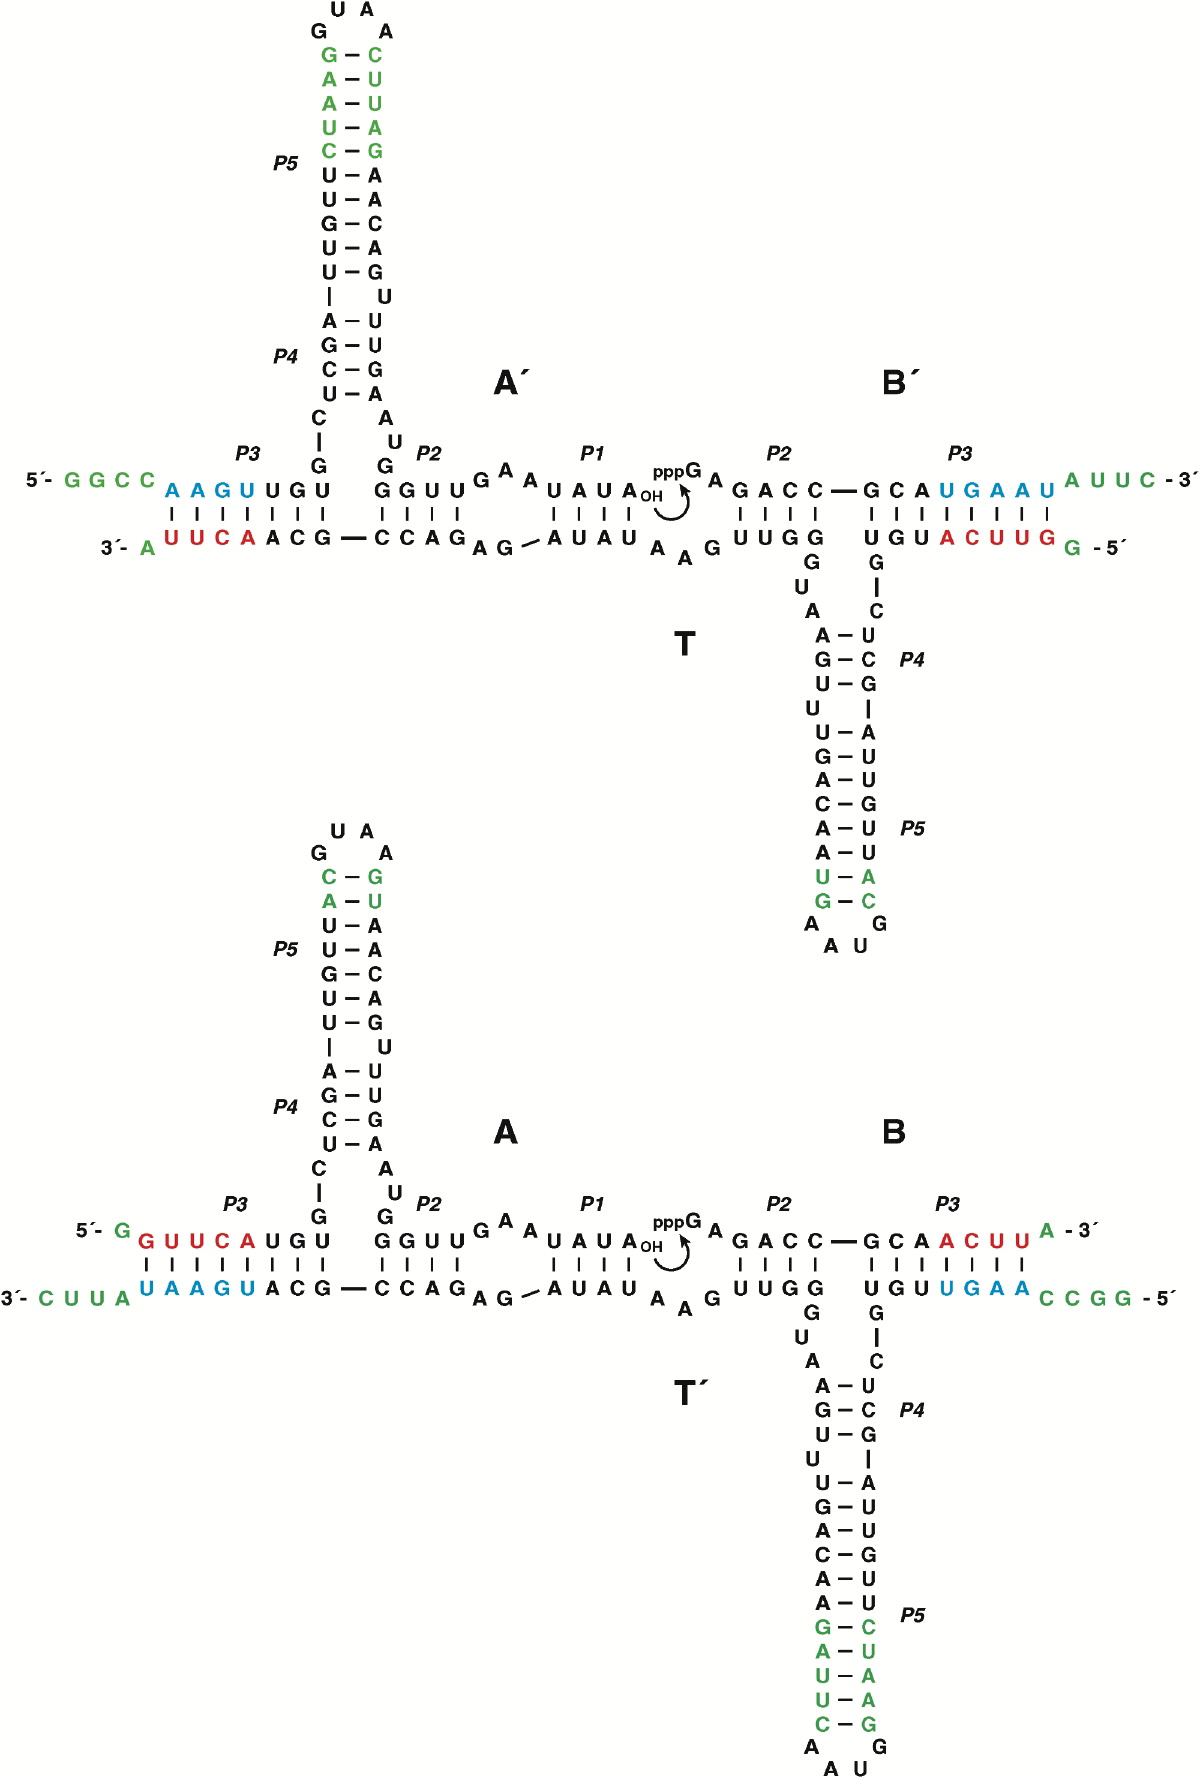
\includegraphics[scale=0.55]{gr3_lrg.jpg}
\caption{Sequence and Secondary Structure of the Ribozymes and Substrates used to Carry Out Cross-Catalytic Replication.\\Taken from \cite{doi:10.1016/j.chembiol.2004.08.021}.}
\label{cross}
\end{figure}
\noindent
As the resulting structure has intramolecular structure in both sequences but independant from each other, we choose mode ``--predMulti=X", for ES values in query or target, to recreate the structure shown in Figure \ref{cross}. Using this mode IntaRNA predicts the exact structure given in the article, see page \pageref{Result:cross}. Furthermore, we tried to run IntaRNA using only parts of the entire sequences to check whether we can still predict the intramolecular structures. The results are shown on page \pageref{Result:split}. The results for the first part of the target sequence are very satisfying, as the intramolecular structure in the target sequence is nearly correct. The second part of the target sequence is likely too short to predict the intramolecular structure in the query.\\
The other structure shown in figure \ref{cross} is the mirrored structure of the first one. Using IntaRNA this structure is also perfectly predicted. The different results for the mirrored structure are shown on page \pageref{Result:mirror}.\\
\begin{landscape}
\begin{spacing}{0.5}
\noindent
{\tiny\texttt{>A}\\
\texttt{GGUUCAUGUGCUCGAUUGUUACGUAAGUAACAGUUUGAAUGGGUUGAAUAUA}\\
\texttt{>B}\\
\texttt{GAGACCGCAACUUA}\\
\texttt{>T = A + B}\\
\texttt{GGUUCAUGUGCUCGAUUGUUACGUAAGUAACAGUUUGAAUGGGUUGAAUAUAGAGACCGCAACUUA}\\
\texttt{>A'}\\
\texttt{GGCCAAGUUGUGCUCGAUUGUUCUAAGGUAACUUAGAACAGUUUGAAUGGGUUGAAUAUA}\\
\texttt{>B'}\\
\texttt{GAGACCGCAUGAAUAUUC}\\
\texttt{>T' = A' + B'}\\
\texttt{GGCCAAGUUGUGCUCGAUUGUUCUAAGGUAACUUAGAACAGUUUGAAUGGGUUGAAUAUAGAGACCGCAUGAAUAUUC}\\
\texttt{>T = A + B}}\\
\end{spacing}
\begin{lstlisting}[style=base]
A' + B' / T structure:
A' + B'
             5                                                                                                     74
             |                                                                                                     |
      5'-GGCC       GCUCGAUUGUUCUAAGGUAACUUAGAACAGUUUGAAUG    GAA    GA                                             AUUC-3'
             @AAGUUGU@                                      @GGUU@   @UAUA@   @GACC@                                @GCAUGAAU@
             @|||||||@                                      @||||@   @||||@   @||||@                                @||||||||@
             @UUCAACG@                                      @CCAG@   @AUAU@   @UUGG@                                @UGUACUUG@
         3'-A                                                 AG     AAG    GUAAGUUUGACAAUGAAUGCAUUGUUAGCUCG        G-5'
             |                                                                                                     |
            65                                                                                                     2
T

Prediction of IntaRNA using --pred=M --mode=E --predMulti=X --noSeed
A' + B'
             5                                                                                                     74
             |                                                                                                     |
      5'-GGCC       GCUCGAUUGUUCUAAGGUAACUUAGAACAGUUUGAAUG    GAA    GA                                             AUUC-3'
             @AAGUUGU@                                      @GGUU@   @UAUA@   @GACC@                                @GCAUGAAU@
             @||||||:@                                      @|||:@   @||||@   @:|||@                                @:||||||:@
             @UUCAACG@                                      @CCAG@   @AUAU@   @UUGG@                                @UGUACUUG@
         3'-A                                                 AG     AAG    GUAAGUUUGACAAUGAAUGCAUUGUUAGCUCG        G-5'
             |                                                                                                     |
            65                                                                                                     2
T
\end{lstlisting}
\label{Result:cross}
\end{landscape}
\newpage
\begin{landscape}
\begin{lstlisting}[style=base]
A' + B' / T structure:
A' + B'
             5                                                                                                     74
             |                                                                                                     |
      5'-GGCC       GCUCGAUUGUUCUAAGGUAACUUAGAACAGUUUGAAUG    GAA    GA                                             AUUC-3'
             @AAGUUGU@                                      @GGUU@   @UAU@$A$   @G@$AC$@C@                                @GCAUGAAU@
             @|||||||@                                      @||||@   @|||@$|$   @|@$||$@|@                                @||||||||@
             @UUCAACG@                                      @CCAG@   @AUA@$U$   $UUGG$                                @UGUACUUG@
         3'-A                                                 AG     AAG    GUAAGUUUGACAAUGAAUGCAUUGUUAGCUCG        G-5'
             |                                                                                                     |
            65                                                                                                     2
T

Prediction of IntaRNA using -q=T -t=A' --pred=M --mode=E --predMulti=X --noSeed
A'
             5                                                     59
             |                                                     |
      5'-GGCC       GCUCGAUUGUUCUAAGGUAACUUAGAACAGUUUGAAUG    GAA   A-3'
             @AAGUUGU@                                      @GGUU@   @UAU@
             @||||||:@                                      @|||:@   @|||@
             @UUCAACG@                                      @CCAG@   @AUA@
         3'-A                                                 AG    UAAG...UGG-5'
             |                                                     |
            65                                                     50
T

Prediction of IntaRNA using -q=T -t=B' --pred=M --mode=E --predMulti=X --noSeed
B'
             1            14
             |            |
          5'-   AC         AUUC-3'
             {GA}@G@  @CGCAUGAAU@
             {|||  |}@:||||||:@
             {CUC  G}@UGUACUUG@
3'-AUU...UUAG              G-5'
             |            |
            13            2
T

\end{lstlisting}
\label{Result:split}
\end{landscape}
\newpage
\begin{landscape}
\begin{lstlisting}[style=base]
A + B / T' structure:
A + B
	 5'-G        GCUCGAUUGUUACGUAAGUAACAGUUUGAAUG    GAA     GA                                                 A-3'
	     @GUUCAUGU@                                @GGUU@   @UAUA@   @GACC@                                      @GCAACUU@ 
	     @||||||||@                                @||:|@   @|:||@   @||||@                                      @|||||||@
	     @UAAGUACG@                                @CCAG@   @AUAU@   @UUGG@                                      @UGUUGAA@
      3'-CUUA                                            AG     AAG    GUAAGUUUGACAAGAUUCAAUGGAAUCUUGUUAGCUCG       CCGG-5'
T'

Prediction of IntaRNA using --pred=M --mode=E --predMulti=X --noSeed
A + B
             2                                                                                                     65
             |                                                                                                     |
         5'-G        GCUCGAUUGUUACGUAAGUAACAGUUUGAAUG    GAA    GA                                                  A-3'
             @GUUCAUGU@                                @GGUU@   @UAUA@   @GACC@                                      @GCAACUU@
             @:||||||:@                                @|||:@   @||||@   @:|||@                                      @:||||||@
             @UAAGUACG@                                @CCAG@   @AUAU@   @UUGG@                                      @UGUUGAA@
      3'-CUUA                                            AG     AAG    GUAAGUUUGACAAGAUUCAAUGGAAUCUUGUUAGCUCG       CCGG-5'
             |                                                                                                     |
            74                                                                                                     5
T'

Prediction of IntaRNA using -q=T' -t=A --pred=M --mode=E --predMulti=X --noSeed
A
             2                                                 52
             |                                                 |
         5'-G        GCUCGAUUGUUACGUAAGUAACAGUUUGAAUG    GAA    -3'
             @GUUCAUGU@                                @GGUU@   @UAUA@
             @:||||||:@                                @|||:@   @||||@
             @UAAGUACG@                                @CCAG@   @AUAU@
      3'-CUUA                                            AG     AAGU...CGG-5'
             |                                                 |
            74                                                 57
T'

Prediction of IntaRNA using -q=T' -t=B --pred=M --mode=E --predMulti=X --noSeed
B
             1           13
             |           |
          5'-   AC        A-3'
             {GA}@G@  @CGCAACUU@
             {|||  |}@:||||||@
             {CUC  G}@UGUUGAA@
3'-CUU...UUAG             CCGG-5'
             |           |
            15           5
T'

\end{lstlisting}
\label{Result:mirror}
\end{landscape}
%An additional case occurs when no structure is enforced to the interaction site.
%\begin{figure}[H]
%\centering
%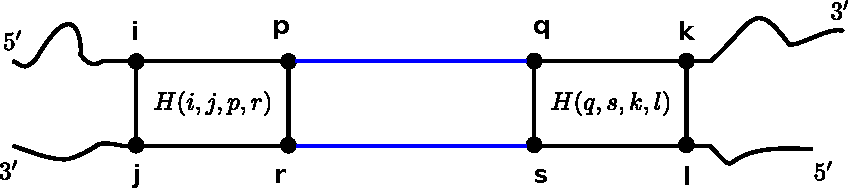
\includegraphics[scale=0.75]{RNAi4.pdf}
%\end{figure}
%\noindent
%To handle this case we can introduce a maximal number of unpaired bases. For the case without structure this is equal to the maximal loop size restriction. But this simplification is also reasonable for the unpaired bases inside a multiloop, because it is not likely to have long chains of unpaired bases in multiloops. We can use this to improve the complexity of our recursions.\\
%\begin{enumerate}
%\item
%\item
%\item
%\item
%\end{enumerate}
%TODO Die Kondition mit der maximal anzahl oben rausnehmen und hier als verbesserung einfügen, die durch die Erkenntnis ensteht dass die Region unstrukturiert sein kann.
\bibliographystyle{plainnat}
\bibliography{intarna2-multi}
%\textbf{RNA}: An RNA molecule is transcribed from a large part of the DNA. It is then translated to proteins. But only a very small part of the RNA encodes for proteins. The other part has regulatory functions inside the cell. The functions of the RNA molecules are directly related to their 3D-structure.\\\\
%\textbf{cRNA}: Coding RNA is translated to proteins. For example the messenger RNA (mRNA) that carries the information to encode proteins.\\\\
%\textbf{ncRNA}: Non-coding RNA, also called non-protein-encoding RNA, performs different functions inside the cell. For example the transfer RNA (tRNA) that delivers amino acids to the ribosome or the ribosomal RNA that binds the amino acids together to form protein chains.\\\\ most algorithms. The sequence encodes biological informatio
%\textbf{bacterial sRNA}: Bacterial small RNAs are highly structured small-chained ncRNAs produced by bacteria. They can have multiple functions, such as the modification of the function of proteins or regulate gene creation by binding to mRNA.\\\\
%\textbf{RNA sequence S}: The RNA sequence S is a chain of bases (Adenine A, Guanine G, Cytosine C and Uracil U). It is used as the primary input ofn and can be folded into a structure to determine the function of an RNA molecule. The RNA sequence is usually ordered from the left end $5^\prime$ to the right end $3^\prime$.
%\begin{figure}[H]
%\centering
%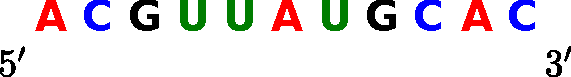
\includegraphics[scale=1]{seqExample.pdf}
%\end{figure}
%\noindent\textbf{RNA structure P}: The functions of ncRNAs are determined by their unique tertiary structures. Due to the hard complexity of tertiary structure prediction, we analyse secondary structures. There are different types of RNA structures. Nested structures containing no pseudoknots and crossing structures that contain pseudoknots, as shown in figure \ref{Nested}.
%\begin{figure}[H]
%\centering 
%
\includegraphics[scale=0.6]{NestedCrossing.pdf}
%\caption{Linear Feynman Diagrams of a nested and a crossing structure.}
%\label{Nested}
%\end{figure}
%\noindent
%The structure is created by bases forming base-pairings by hydrogen bonds. The standard base pairs, the Watson-Crick base pairs, are G-C, A-U, C-U, due to their high binding strength.\\\\
%\begin{figure}[H]
%\centering
%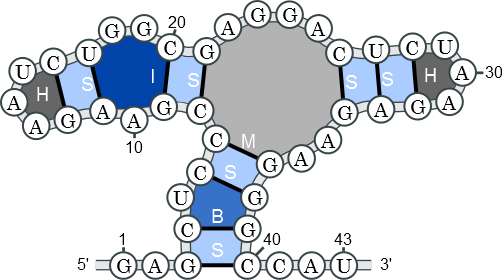
\includegraphics[scale=0.5]{structure-loops.png}
%\caption{Overview of structure elements. \citep{ELearn}}
%\label{Structure}
%\end{figure}
%\noindent
%There are different structural elements that are formed by the binding of base pairs. These elements are the hairpin loops (H), stackings (S), internal/bulge loops (I/B) and multiloops (M), as shown in figure \ref{Structure}.\\
%A secondary structure is composed of these structural elements.\\\\
%\textbf{Structure ensemble}: The structure ensemble $\mathcal{S}$ is the set of all structures that can be formed from sequence S.\\\\
%The quality of an RNA-RNA interaction between two subsequences $s_{i}^1 ... s_{k}^1$ and $s_{j}^2 ... s_{l}^2$ is determined by its hybridisation energy $H(i,j,k,l)$ and the accessibility of the interaction site.
%TODO cite
%\cite{Andreas}
%$H(i,j,k,l)$ denotes the hybridisation energy of the best interaction of subsequence $s_{i}^1 ... s_{k}^1$ and $s_{j}^2 ... s_{l}^2$ where $(i,j)$ and $(k,l)$ form base pairs.\\
%\begin{equation*}
%C(i,j,k,l) =  \begin{cases}
%						\min\limits_{p,q,r,s} 
%						\begin{rcases}
%						\begin{dcases} 
%						EHA + ES(p,q)+ a + b + (s-r-1)\cdot c\\
%						EHA + ES(r,s)+ a+b+(q-p-1)\cdot c\\
%						EHA + ES(p,q) + ES(r,s) + a + b\\
%						\end{dcases}
%						\end{rcases} &(\seq_i^1,\seq_j^2) \text{ and } (\seq_k^1,\seq_l^2) \text{ pair,}\\
%   						\infty &\text{ otherwise.}\\
%			  \end{cases}\\
%\end{equation*}
\end{document}
